\documentclass[fontsize=12pt, a4paper]{scrartcl}
\let\stdsection\section 	% neue seite für neues kapitel
\renewcommand\section{\newpage\stdsection} 

% ### variables

\def \var_single_plot_width {0.49}
\def \var_double_plot_width {0.49}

% ### literaturverzeichnis
\usepackage[sorting=none]{biblatex}
\addbibresource{sim_axelsson.bib}

% ### sprachpakete
\usepackage[ngerman]{babel} % Deutsche Sprachanpassungen
\usepackage[T1]{fontenc}    % Silbentrennung bei Sonderzeichen
\usepackage[utf8]{inputenc} % Direkte Angabe von Umlauten im Dokument.
    
% ### grafiken   
\usepackage{graphicx}		% Zur Darstellung von Bildern
\usepackage{subcaption}
\usepackage{float}			% platziert figures am gewünschten platz
\usepackage[export]{adjustbox}% http://ctan.org/pkg/adjustbox

% ### matplotlib plots
\usepackage{pgf}
\usepackage{lmodern}% http://ctan.org/pkg/lm
%\usepackage{tikz}
\usepackage{pgfplots}
\pgfplotsset{width=10cm,compat=1.9}
%\pgfplotsset{compat=newest}

\usepackage{csquotes}

\usepackage[parfill]{parskip}

% ### curcuits
\usepackage{tikz}
\usetikzlibrary{arrows}
\usepackage[RPvoltages]{circuitikz}

% ### titleseite
\usepackage{titling}
\title{Systemmodelierung einer Membranpump für die Mikro-Fluidik}
\author{Kristjan Axelsson, Timo Stubler}
\date{\today}               

% ### fancy features
\usepackage{hyperref}

\begin{document}
\pagenumbering{gobble}		% turn off page numbers
\begin{titlingpage}
\begin{center}
\begin{figure}[H]
    \centering
    \begin{subfigure}[B]{0.2\textwidth}
        
\includegraphics[width=\textwidth, valign=t]{bilder/Logo_MNM_EN_Farbe_ohneHM (1).png}
    \end{subfigure}
    \begin{subfigure}[B]{0.45\textwidth}
        
\includegraphics[width=\textwidth, valign=t]{bilder/Hochschule_Muenchen_Logo.png}
    \end{subfigure}
\end{figure}
\setcounter{figure}{0}
\vspace{2cm}
\begin{large} 
\textbf{\thetitle} \\
\end{large}
\vspace{1cm}
\theauthor\\
\vspace{1cm}
Hochschule München \\
Fakultät für angewandte Wissenschaften und Mechatronik \\
\vspace{1cm}
\thedate
\end{center}
\end{titlingpage}

\tableofcontents            % Inhaltsverzeichnis anlegen

% quelle \cite{pedrotti} \\
% siehe Abb. \ref{fig_detector_test} \\
% siehe Kap. \ref{fazit}

\section{Einleitung}
\pagenumbering{arabic}		% turn on page numbers

\section{Theorie}

\section{Gegendruck}

\begin{figure}[H]
    \centering
    \begin{subfigure}[H]{0.4\textwidth}
        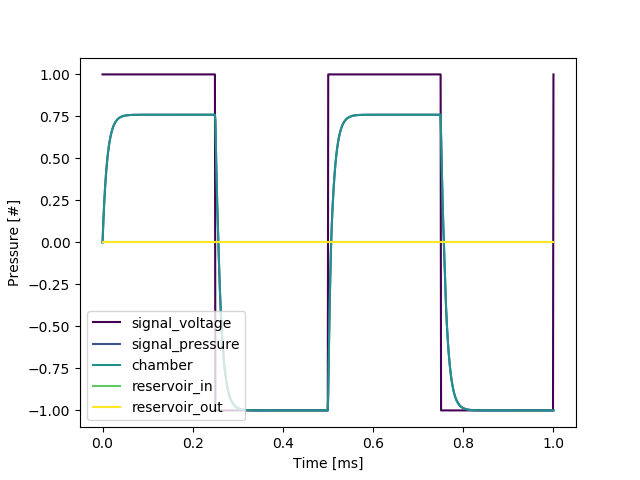
\includegraphics[width=\textwidth, valign=t]{bilder/backpressure/backpressure_free.png}
        \caption{•}
    \end{subfigure}
    \begin{subfigure}[H]{0.4\textwidth}
        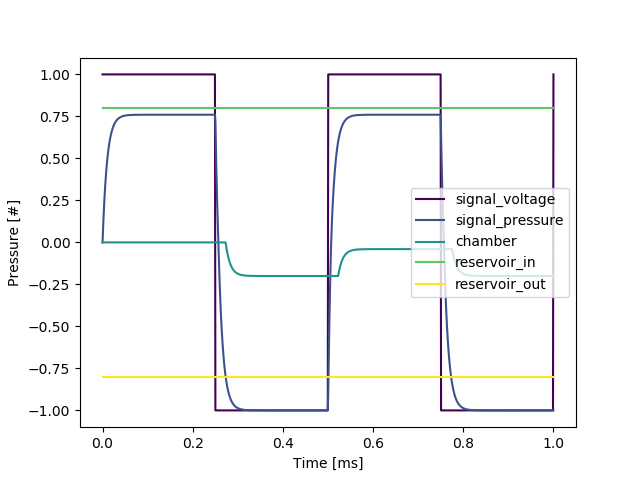
\includegraphics[width=\textwidth, valign=t]{bilder/backpressure/backpressure_example.png}
        \caption{•}
    \end{subfigure}
    \caption{•}
\end{figure}

\begin{figure}[H]
    \centering
    \begin{subfigure}[H]{0.4\textwidth}
        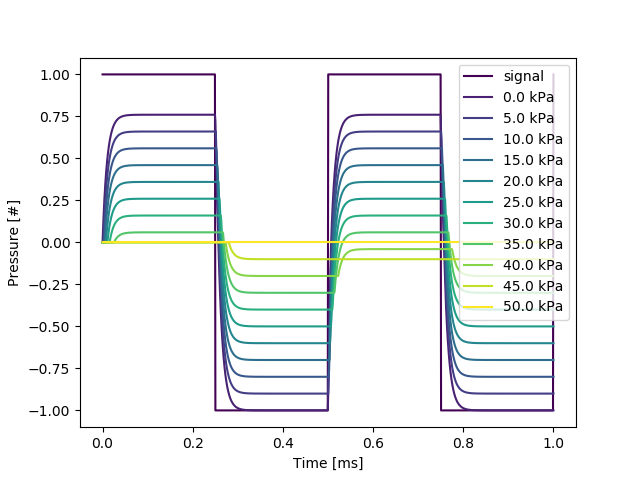
\includegraphics[width=\textwidth, valign=t]{bilder/backpressure/backpressure_at_pr_in_and_pr_out.png}
        \caption{•}
    \end{subfigure}
    \begin{subfigure}[H]{0.4\textwidth}
        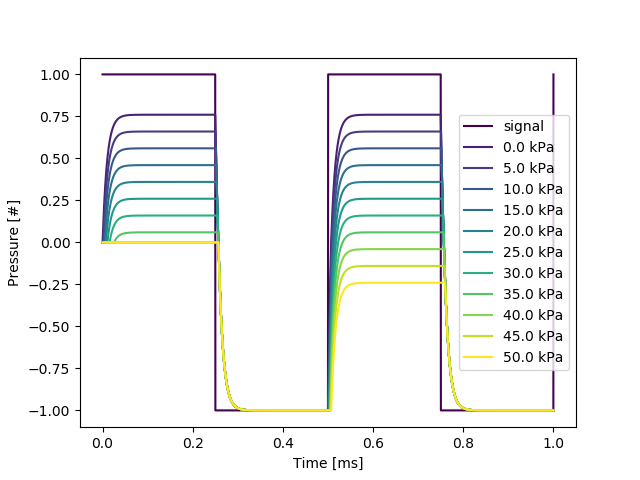
\includegraphics[width=\textwidth, valign=t]{bilder/backpressure/backpressure_at_pr_in.png}
        \caption{•}
    \end{subfigure}
    \caption{•}
\end{figure}



\begin{figure}[H]
	\centering
	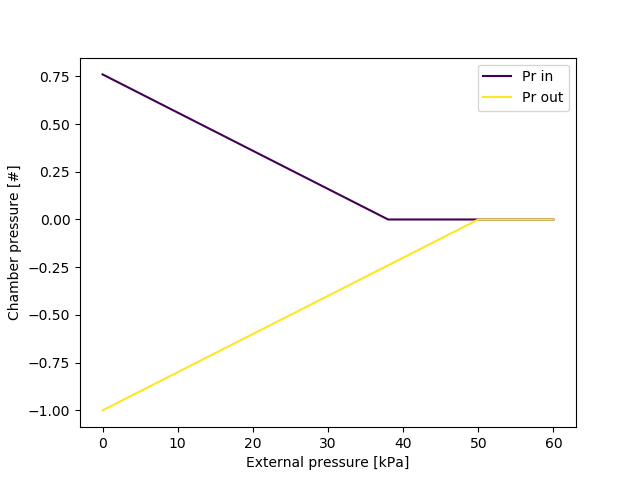
\includegraphics[width=0.7\textwidth]{bilder/backpressure/backpressure_result.png}
	\caption{•}
\end{figure}

\section{Grenzfrequenz}


\begin{figure}[H]
    \centering
    \begin{subfigure}[H]{0.4\textwidth}
        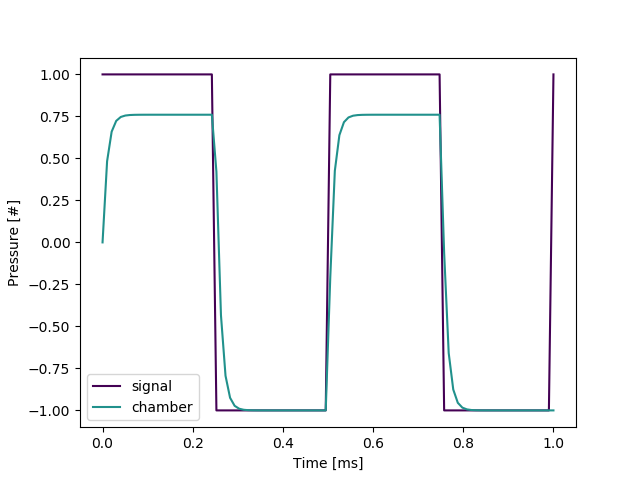
\includegraphics[width=\textwidth, valign=t]{bilder/frequency/frequency_default_2kHz.png}
        \caption{•}
    \end{subfigure}
    \begin{subfigure}[H]{0.4\textwidth}
        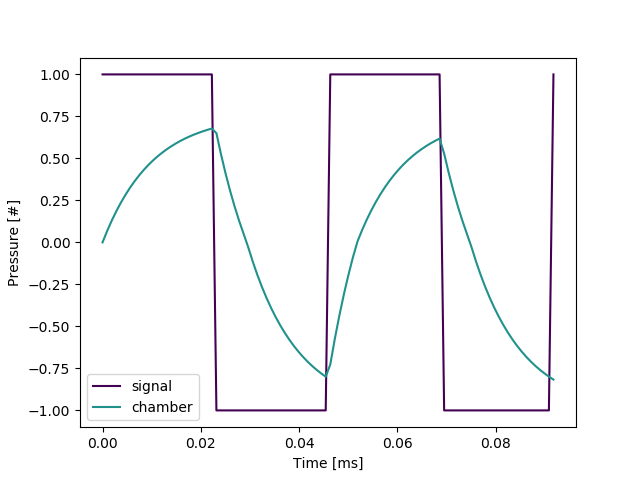
\includegraphics[width=\textwidth, valign=t]{bilder/frequency/frequency_to_fast_21_8 khz.png}
        \caption{•}
    \end{subfigure}
    \caption{•}
\end{figure}

\begin{figure}[H]
    \centering
    \begin{subfigure}[H]{0.4\textwidth}
        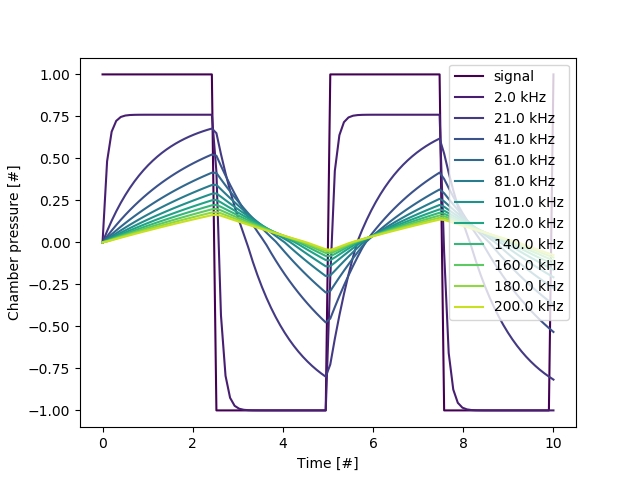
\includegraphics[width=\textwidth, valign=t]{bilder/frequency/frequency_sweep.png}
        \caption{•}
    \end{subfigure}
    \begin{subfigure}[H]{0.4\textwidth}
        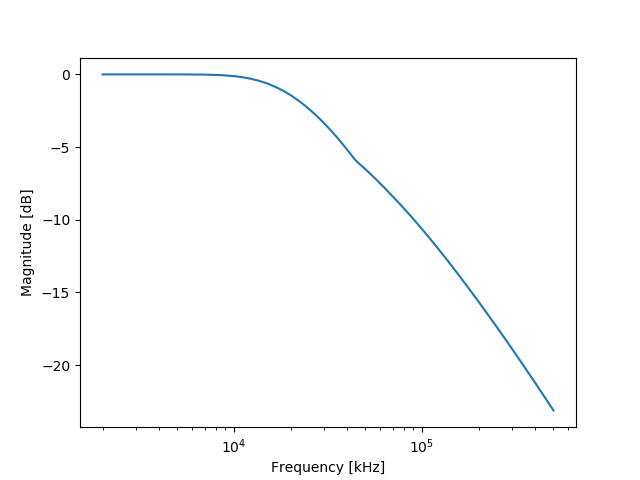
\includegraphics[width=\textwidth, valign=t]{bilder/frequency/bode_diagram.png}
        \caption{•}
    \end{subfigure}
    \caption{•}
\end{figure}


\printbibliography

\end{document}
